\section{引力势能}\label{sec:06.03}

在\ref{sec:06.01}节,我们曾指出,地面附近的质点具有重力势能$ mgz $,
现在更一般地讨论万有引力势能。

\begin{wrapfigure}[9]{r}{13em}
  \vspace{-2em}
  \centering
  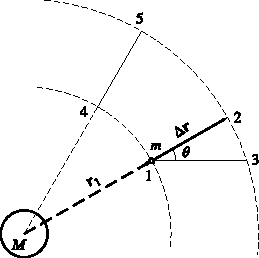
\includegraphics{figure/fig06.06}
  \caption{引力作的功}
  \label{fig:06.06}
\end{wrapfigure}
如图\ref{fig:06.06}\;所示,物体$ M $对质点$ m $的万有引力在二者连线方
向,大小为%\vspace{-0.4em}
\begin{equation*}
  F = G \frac { m M } { r ^ { 2 } }
\end{equation*}
如果我们将$ m $沿着连线方向(图\ref{fig:06.06}\;中是径向方向)从1移至2,即
从$ \vec{r} _ 1 $到$ \vec{r} _ 2 \left( \vec{r} _ 2 = \vec{r} _ 1 + \Delta \vec{r} \right) $,当移动
距离$ \Delta \vec{r} $很小时,引力$ F $作的功近似为
% 174.jpg
%\clearpage\mbox{}\vspace{-1.56em}
\begin{equation*}
  A = \vec{F} \cdot \Delta \vec{r} = - G \frac { m M } { r _ 1 ^ { 2 } } \Delta r
\end{equation*}
负号是由于力的方向与位移方向反平行。再考虑$ m $从1移到3,在
这条路径上力与位移夹角为$ \left( \uppi - \theta \right) $,而位移大小为$ \Delta r / \cos \theta $,所以
引力功近似为
\begin{equation*}
  \begin{aligned}
    A & = \vec{F} \cdot \dif \vec{r}                                                                                        \\
      & = \frac { G m M } { r _ { 1 } ^ { 2 } } \cdot \frac { \Delta r } { \cos \theta } \cdot \left( - \cos \theta \right) \\
      & = - G \frac { m M } { r _ 1 ^ { 2 } } \Delta r
  \end{aligned}
\end{equation*}
而在从3移到2的路径上,引力总是与位移垂直,所以不作功。因
此,我们证明了路径$1 \to 3 \to 2$引力作功与相应的径向路径$ 1 \to 2 $上引
力作功相同,这是万有引力作功的第一个性质。再则,按图6.6,
如果$ 4 $及$ 5 $与$ M $的距离也分别是$ r_1 $,$ r_2 $,并且$ 4 \to 5 $在径向方向,那么
引力在$ 4 \to 5 $的路径上所作的功与在$ 1 \to 2 $上所作的功相同,因为引
力的大小只与$ m $及$ M $之间的距离有关,而与方向无关。这是引力
作功的第二个性质。

有了上述两点,现在可以进行下面的证明:如图\ref{fig:06.07},当质点
\begin{wrapfigure}[9]{r}{17em}
  \vspace{-1.3em}
  \centering
  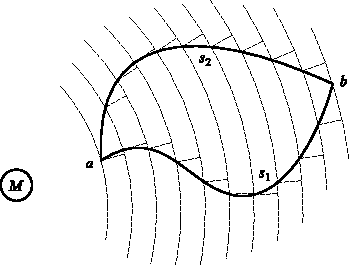
\includegraphics{figure/fig06.07}
  \caption{引力作功与路径无关}
  \label{fig:06.07}
\end{wrapfigure}
由$ a $运动到$ b $时,对于任意两条路径,如$ s _ { 1 } $及$
  s _ { 2 } $,万有引力作功相同。首先画出一系列与
$ M $等距的面,在图上用虚线圆弧表示,它们将
$ s _ { 1 } , s _ { 2 } $分割成许多非常
小的小段,这些小段可以认为是直线。然后在每个小段处画出相应的
% 175.jpg
径路径,图上用径向虚线段表示。现在,用上面所证明的第一
个性质可得,在$ s _ { 1 } $或$ s _ { 2 } $上作的功与图中各相应的所有径向小段上
作功的总和相等。再利用上述第二个性质,即得在$ s _ { 1 } $ 及$ s _ { 2 } $的相应
径向小段上作功相等,因而沿$ s _ { 1 } $及$ s _ { 2 } $引力作功相等。

读者可能还会认为,$ s _ { 2 } $并不够一般,如果取图6.8中那样的$ s _ { 3 } $
结果如何?用同上的方法,不难证明,沿着$ s _ { 3 } $由$ a $到$ b $与沿$ s _ { 1 } $由
$ a $到$ b $,引力作功相等。因为在从$ a $到$ c $和从$ c $到$ d $各对应小段上,
功的绝对值相同,但由于位移方向相反,故其功正好相互抵消,
所以在沿$ s _ { 3 } $由$ a $到$ c $再到$ d $,引力作功为零。因此,沿$ s _ { 1 } $或$ s _ { 3 } $由
$ a $到$ b $,引力作功仍然相同。

\begin{figurex}
  \centering
  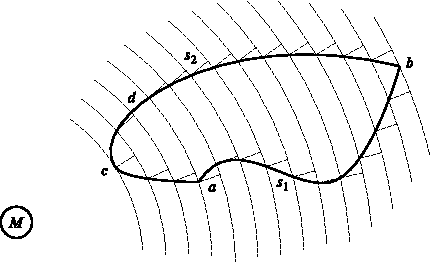
\includegraphics{figure/fig06.08}
  \caption{引力作功与路径无关}
  \label{fig:06.08}
\end{figurex}

这样,我们证明了万有引力作功与路径无关的基本性质。因
此,由$ a $到$ b $,引力作功可写为
\begin{equation}\label{eqn:06.03.01}
  \begin{aligned}
    A & = \int \limits _{(l)} F \cdot \dif \vec{r} = \int _ { \vec{r}_a } ^ { \vec{r}_b } \vec{F} \cdot \dif \vec{r} = - \int _ { r _ a } ^ { r _ b } \frac { G m M } { r ^ { 2 } } \dif r \\
      & = \frac { G m M } { r _ { b } } - \frac { G m M } { r _ { a } }
  \end{aligned}
\end{equation}

% 176.jpg
\clearpage
根据功的定义,我们有
\begin{equation}\label{eqn:06.03.02}
  A = T _ { b } - T _ { a }
\end{equation}
由式\eqref{eqn:06.03.01}、\eqref{eqn:06.03.02},可得
\begin{equation*}
  \frac { G m M } { r _ { b } } - \frac { G m M } { r _ { a } } = T _ { b } - T _ { a }
\end{equation*}
或\vspace{-1.56em}
\begin{equation}\label{eqn:06.03.03}
  \begin{aligned}
      & T _ { a } + \left( - \frac { G m M } { r _ { a } } \right)                 \\
    = & T _ { b } + \left( - \frac { G m M } { r _ { b } } \right) = \text{不变量}
  \end{aligned}
\end{equation}
由式\eqref{eqn:06.03.03}看到,我们找到了质点在引力作用下的一个不变量。
因为$ a $,$ b $是任意的,所以式\eqref{eqn:06.03.03}可一般地写为
\begin{equation}\label{eqn:06.03.04}
  T + \left( - \frac { G m M } { r } \right) = \text{不变量} = E
\end{equation}

我们定义
\begin{equation}\label{eqn:06.03.05}
  V \equiv - \frac { G m M } { r }
\end{equation}
为引力势能,则$ E $就是总机械能。式\eqref{eqn:06.03.04}就是我们前面讲过的
机械能守恒定律在引力场中的表达式。

以上讨论的关键点是引力作功与路径无关,正是由于这一点,
我们才有可能定义引力势能。

再次指出,式\eqref{eqn:06.03.04}所描写的物理性质并没有超出动力学基
本方程$ \vec{F} = m \vec{a} $。原则上讲,动力学方程已包括式\eqref{eqn:06.03.04}。但在处
理某些问题时,直接用式\eqref{eqn:06.03.04}会更加简便,更容易看清物理的
实质。下面举几个实例来说明这一点。

根据式\eqref{eqn:06.03.05},可以画出引力势能与径向位置的关系,如图
6.9所示。从图中容易看出,当$ r \to \infty $时,引力势能趋于零。由这
幅图,我们可以很方便地讨论许多问题。

我们知道,质点在引力作用下运动时的总能量$ E $是常数,即
% 177.jpg
\begin{equation*}
  E = \frac { 1 } { 2 } m v ^ { 2 } - \frac { G m M } { r } = \text{不变量}
\end{equation*}
因此,在上图中,$ E $是一条平行于$ r $轴的直线。由于动能不可为
负,所以当$ E < 0 $时,$ m $与$ M $间的最大距离应为
\begin{equation*}
  r _ { \max } = \frac { G m M } { | E | }
\end{equation*}
\begin{wrapfigure}[10]{r}{17em}
  \vspace{-1.3em}
  \centering
  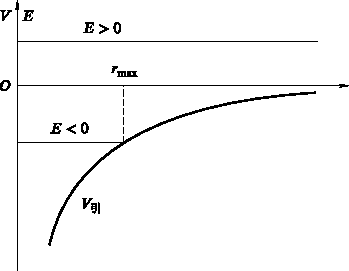
\includegraphics{figure/fig06.09}
  \caption{引力势能}
  \label{fig:06.09}
\end{wrapfigure}
从图6.9中容易看出,当$ E < 0 $时,质点只能在
$ r = 0 $到$ r = r _ { \max } $之间运动,这种运动称为束缚
运动。当$ E \geqslant 0 $,$ E $线在横轴以上,它不与$ V_\text{引} $
线相交。所以质点可以在$ r = 0 $到$ \infty $的整个范围
里运动。这种运动称为自由运动。

由图\ref{fig:06.09}\;不难求出
第二宇宙速度,即从地球发射的人造行星所需要的最低速度。人
造行星是逃离地球引力作用的东西,也就是说它对地球引力已成
为自由运动。因此,在这种情况总机械能$ E $至少为零,所以在发
射时,它的速度至少应为
\begin{equation*}
  \frac { 1 } { 2 } m v ^ { 2 } - \frac { G m M _ \text { 地 } } { R } = 0
\end{equation*}
其中$ R $为地球半径。故
\begin{equation*}
  v = \sqrt{\frac { 2 G M _ \text{地} } { R } }
\end{equation*}
由于$ g = \dfrac { G M _ \text{地} } { R ^ { 2 } } $,所以
% 178.jpg
\clearpage
\begin{equation*}
  \begin{aligned}
    v & = \sqrt { 2 g R } \approx \left( 2 \times 10 \times 6.4 \times 10 ^ { 6 } \right) ^ { \frac { 1 } { 2 } } \\
      & \approx 11.3 \times 10 ^ { 3 } \text{米/秒}
  \end{aligned}
\end{equation*}

下面我们讨论宇宙飞船从地球飞往月球的问题。图6.10给出
地-月系统的势能图。如果飞船的发射速度过低,即$ E $小,则飞
船只能在地球附近运动,不可能到达月球;发射速度过高,即$ E $
大,飞船也不会落到月球引力束缚范围,而可能远离地-月体系,
成为太阳的行星。因此发射能量只能控制在如图所示的非常小的
可调范围内,才能离开地球到达月球引力束缚的范围,然后再设
法进一步减速,落到月球上。再有,不仅要把发射能量控制在一个
非常窄的范围内,还必须把飞行轨道控制在一个非常小的空间区
域里,才能到达月球。

\begin{figurex}
  \centering
  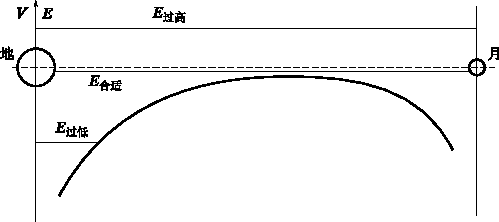
\includegraphics{figure/fig06.10}
  \caption{地-月系统势能图}
  \label{fig:06.10}
\end{figurex}

最后应当指出,引力势能实际上是属于$ m $及$ M $二者组成的体
系的,因势能决定于二者之间的相对距离。其他的势能也有同样
特点,也应是属于一个体系的。物体在不同高度上的重力势能,
确切地说应是属于物体及地球组成的体系的,但由于在这势能转
化过程中地球的运动状态的改变完全可以不计,所以我们可以采
用“物体的重力势能”这种虽不确切但完全适用的说法。

宇宙间的物质都参与万有引力的作用,引力势能是最常见的
% 179.jpg
一种能量形式。就宇宙范围来说,自然界的大部分能量,都是以
引力势能形式存在的。